\begin{frame}{Experiment 1}
\setbeamercovered{invisible}
\fontsize{11pt}{15}\selectfont
\textbf{Tool use} and \textbf{syntax} rely on \textbf{neural activity} within common anatomical territories in the BG.\\ %Brain activity displays similar spatial distribution
\begin{figure}
    \centering
    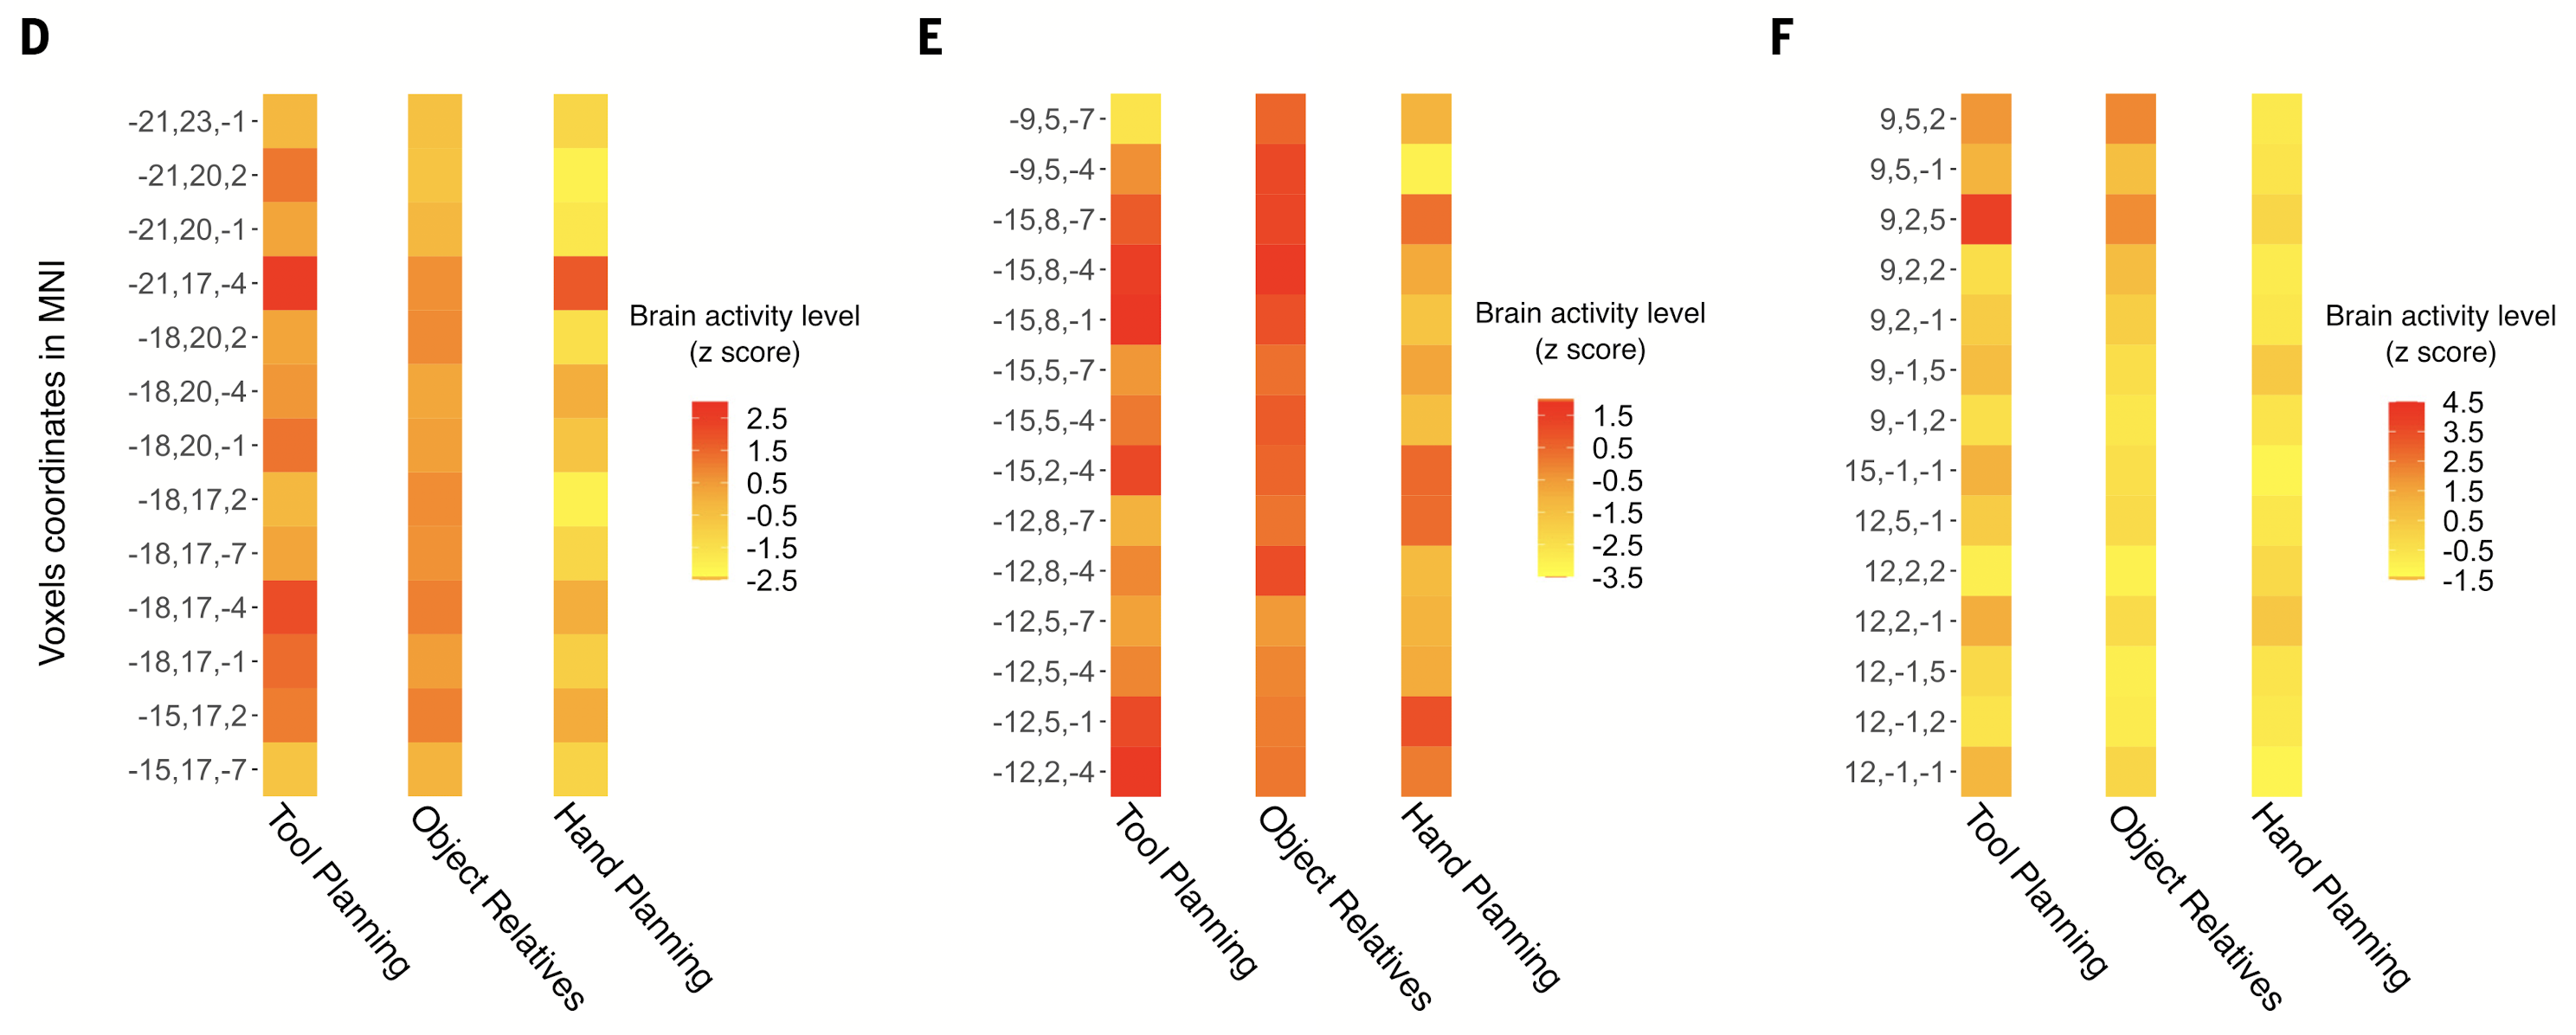
\includegraphics[width=10.5cm]{images/paper_pics/fig2DEF.png}
    \caption*{Spatial distribution of neural activity for tool-use planning, object-relative planning, and free-hand planning in the BG. Each single colored square represents a single voxel for the lCau (D), lGPi (E), and rGPi (F).}
    \label{fig:label5}
\end{figure}

\end{frame}